Measures relations are defined by their similarity. This similarity is called the measure match rate. The match rate is calculated by the Levenshtein distance \cite{Levenshtein} to get a ratio between 0 and 1 that represents the similarity between two measures.
On figure \ref{fig:GF_measures}, the 9th and 10th measure of the Godfather theme song are portrayed. The following is an example of match rates of the two measures.
\begin{figure}[H]
	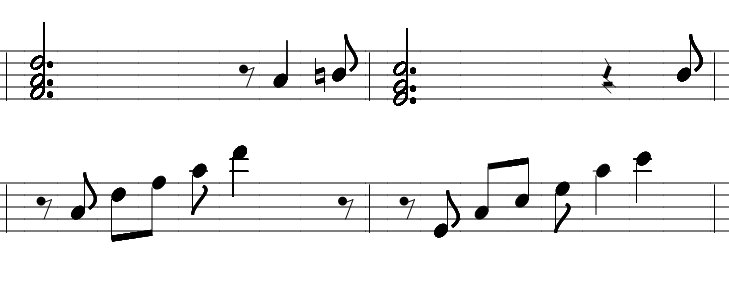
\includegraphics[width=\linewidth]{Fotos/measures/GF_9-10.png}
	\caption{The 9th and 10th measure of the Godfather theme song.}
	\label{fig:GF_measures}
\end{figure}
\[\textit{TYPES}\]
\[A: [X, N, N, N, N, N, N, N] \]
\[B: [X, N, N, N, N, N, N, N] \]
\[\textit{types match rate}: 100\% \]

\[\textit{PITCHES}\]
\[A: [E\flat4C5G4, G2, C3, E\flat3, G3, C4, E\flat4, B\flat4] \]
\[B: [D5G\sharp4F4, C3, F3, G\sharp3, C4, F4, G\sharp4, B4] \]
\[\textit{pitches match rate}: 74\% \]

\[\textit{DURATIONS}\]
\[A: [complex, eighth, eighth, eighth, eighth, \]
\[quarter, quarter, eighth] \]
\[B: [complex, eighth, eighth, eighth, eighth, \]
\[quarter, quarter, eighth]\]
\[\textit{durations match rate}: 100\% \]

\[\textit{OFFSETS}\]
\[A: [0.0, 0.5, 1.0, 1.5, 2.0, 2.5, 3.0, 3.5]\]
\[ B: [0.0, 0.5, 1.0, 1.5, 2.0, 2.5, 3.0, 3.5] \]
\[\textit{offsets match rate}: 100\% \]

\[\textit{SEMITONES}\]
\[ A: [-20, 5, 3, 4, 5, 3, 7] \]
\[ B: [-26, 5, 3, 4, 5, 3, 3]\]
\[\textit{semitones match rate}: 91\% \]

\[\textit{COMBINED}\]
\[ A: [XE\flat4C5G4c0.0, NG2e0.5, NC3e1.0, NE\flat3e1.5, \]
\[NG3e2.0, NC4q2.5, NE\flat4q3.0, NB\flat4e3.5]\]
\[ B: [XD5G\sharp4F4c0.0, NC3e0.5, NF3e1.0, NG\sharp3e1.5,\]
\[NC4e2.0, NF4q2.5, NG\sharp4q3.0, NB4e3.5]\]
\[\textit{combined match rate}: 85\% \]